\section{Introduction}\label{introduction}

Fachechi, Agliari and Barra \supercite{fachechi2019dreaming} (Neural
Networks 112, 2019, 24--40; arXiv:1810.12217) revisit the ``unlearning''
idea of Hopfield, Feinstein and Palmer \supercite{hopfield1983unlearning}
and derive a closed-form ``dreaming'' kernel for the Hopfield model.
Starting from the Hebbian coupling matrix
\(J = \frac{1}{N}\sum_{\mu=1}^{P}\xi^\mu\xi^{\mu\mathsf T}\) built from
\(P = \alpha N\) random \(\pm1\) patterns, a sleep phase of duration
\(t\) produces

\[J(t) = J\,(1+t)\,(\mathbb 1 + tJ)^{-1},\]

which equals \(J\) at \(t = 0\) and tends to the projection
(pseudo-inverse) rule of Kanter and Sompolinsky
\supercite{kanter1987projector} as \(t \to \infty\). The article's
statistical-mechanics analysis predicts that the critical storage load
\(\alpha_c(t)\) rises from the Amit--Gutfreund--Sompolinsky value
\supercite{amit1985storing} \(\approx 0.138\) at \(t = 0\) towards the
theoretical bound \(\alpha = 1\), that spurious (mixture) attractors are
removed, that pure patterns are reinforced, and that the gain is robust
to thermal noise. The original Monte Carlo checks (Section 2.5 of the
published article) use, for the magnetisation curves, single-spin-flip
Glauber dynamics measured after equilibration on networks of
\(N = 5\,000\) neurons averaged over \(M = 10\) pattern realisations
(their Fig. 7, loads \(P/N \in \{0.02, 0.08, 0.32\}\),
\(t \in \{0, 0.1, 1, 10,
100, 1000\}\)) and a finite-size comparison at \(N \in \{500, 1\,000,
5\,000\}\) (their Fig. 8). The zero-noise internal-field and basin
analyses (their Figs. 9--10) use the \emph{parallel} sign update of
their Eq. (2.17) at \(N = 1\,000\), \(P = 50\): 20 evolutions for each
of 20 pattern realisations for the fields (Fig. 9), 200 evolutions for
each of 200 realisations for the basins (Fig. 10), the cue being the
first pattern with each bit flipped independently with probability \(p\)
and success being declared when that pattern carries the largest Mattis
overlap. The replica-symmetric capacity rises from
\(\alpha_c(0) \simeq 0.138\) to \(\alpha_c \simeq 1.07\) as
\(t \to \infty\), the excess over Gardner's bound being attributed to
replica-symmetry breaking. No capacity curve is measured by Monte Carlo
in the original: the simulations verify magnetisations, fields and
basins against the theory.

We independently implement the published kernel and \emph{partially}
replicate its qualitative claims at finite size (\(N \le 1\,000\)) with
a new, noisy-cue capacity estimator and new random seeds: we test the
retrieval gain, the removal of spurious final states, the robustness to
thermal noise and the projector limit, and we do not reproduce the
replica-symmetric capacity curve nor the original Monte Carlo figures.
Each of the three studies was pre-registered and frozen by an annotated
git tag before its own main run; the later registrations were informed
by the preceding studies (Section ``Pre-registration''). The replication
was carried out inside the Hypneum Lab research programme (issue
hypneum-lab/nerve-wml\#68), where the dreaming kernel serves as a
reference operation; the replication stands on its own and makes no
claim about that programme.

Beyond replicating, we add one control absent from the original work: a
uniform multiplicative rescaling (``downscale'') of the Hebbian
couplings, matched to the dreamed kernel on the Frobenius norm. This
control answers a question the original article does not ask --- whether
the benefit of dreaming could be reproduced by a global reduction of
synaptic strength, as in homeostatic-downscaling accounts of sleep
\supercite{tononi2014shy} --- and it provides a calibrated null for the
capacity ratio. Finally, we test the kernel on correlated patterns,
which the original article treats only for independent patterns.

\section{Methods}\label{methods}

\subsection{Original model}\label{original-model}

Binary units \(s_i \in \{\pm1\}\), \(i = 1 \dots N\); patterns
\(\xi^\mu \in \{\pm1\}^N\) i.i.d. uniform; Hebbian kernel as above;
dreamed kernel \(J(t)\). In pattern space,
\(J_{ij}(t) = \frac1N\sum_{\mu\nu}\xi_i^\mu
[(1+t)(\mathbb 1 + tC)^{-1}]_{\mu\nu}\xi_j^\nu\) with
\(C_{\mu\nu} = \frac1N\xi^\mu\!\cdot\xi^\nu\). The eigenvalues
\(\lambda \ge 0\) of \(J\) map to \(\lambda(1+t)/(1+t\lambda)\).
Retrieval is assessed by the overlap \(m = \frac1N\sum_i s_i\xi_i^\mu\)
of the final state with a stored pattern.

\subsection{Implementation}\label{implementation}

Our code
(\texttt{experiments/nh01\_hopfield\_dream/\{run,confirmatory,correlated\}.py},
713 + 384 + 237 lines, NumPy only, no original code reused) computes
\(J(t)\) by spectral decomposition of the symmetric \(J\)
(\texttt{numpy.linalg.eigh}, negative numerical eigenvalues clipped to
0). Twenty test functions (23 executed cases) check that \(J(0) = J\),
that the spectral form equals the pattern-space closed form on 2-pattern
and many-pattern cases, that \(t = 10^{8}\) approximates the projector
within the tested tolerance, that the matched shrink is exactly inert at
zero temperature
{[}\texttt{code/tests/test\_nh01\_hopfield\_dream.py}{]}, and cover the
confirmatory and correlated runners.

The diagonal \(J_{ii}\) is set to 0 in every arm before the dynamics.
The dynamics are asynchronous with one fresh random permutation of the
\(N\) units per sweep, shared by the probes of a cell. At \(T = 0\),
\(s_i \leftarrow \operatorname{sign}(h_i)\) with ties (\(|h_i| \le
10^{-12} N \max|J|\)) resolved by keeping the current spin --- a
tolerance chosen so that the rule is exactly invariant under
\(J \to cJ\); the run stops at the first sweep without a flip, cap 100
sweeps (non-convergence counted as not retrieved; none occurred in any
run). At \(T = 0.2\), Glauber updates with
\(P(s_i = +1) = 1/(1+e^{-2\beta h_i})\), \(\beta = 5\), 40 sweeps,
overlap averaged over the last 10.

Cue: a stored pattern with exactly \(\operatorname{round}(0.10\,N)\)
bits flipped (overlap 0.80 at \(N = 1\,000\); 0.8125, 0.797, 0.797 at
\(N = 64\), 128, 256 because of rounding). Probes: the first
\(\min(P, 32)\) stored patterns. Final states are classified as
\texttt{retrieved} (\(m \ge 0.9\); \(0.8\) at \(T = 0.2\)),
\texttt{other\_stored} or \texttt{spurious}. Capacity estimator per
(arm, seed): \(\hat\alpha_c\) is the linearly interpolated 0.5 crossing
of the retrieval fraction \(r(\alpha)\) immediately after the
\emph{last} grid load with \(r \ge 0.5\), on the grid
\(\alpha \in \{0.04, 0.06, \dots, 0.20, 0.25, \dots, 0.95\}\) (24
values; 0.01 and 0.02 added for the correlated run). If the largest load
still has \(r \ge 0.5\) the estimate is right-censored at 0.95; if no
load reaches 0.5 the code records the flag \texttt{below\_grid} and a
zero sentinel, which marks censoring, not a measured zero capacity.
Patterns are nested in \(\alpha\) and the same patterns, cues and update
orders are used for every arm of a cell (paired design). Statistics are
paired per-seed ratios and differences, mean over 10 seeds with a 95 \%
percentile bootstrap CI (10 000 seed-level resamples, bootstrap seed
20261025). Every random draw comes from
\texttt{numpy.random.default\_rng({[}20261025,\ seed,\ N,\ stream{]})}.

\subsection{Matched uniform-shrink control
(added)}\label{matched-uniform-shrink-control-added}

For each \(t > 0\), \(J_c = c(t)\,J\) with
\(c(t) = \|\mathrm{offdiag}\,J(t)\|_F / \|\mathrm{offdiag}\,J\|_F\),
i.e. equal global synaptic budget; \(c\) depends on \(t\), \(\alpha\),
\(N\) and the seed, and all observed values lie in \([0.09, 0.999]\).
Two facts were declared before any run so that the control cannot be
misread: at \(T = 0\) the sign dynamics is invariant under \(c > 0\), so
the control must give a ratio of exactly 1 (an implementation check, not
an empirical hypothesis); at \(T > 0\), \(J_c\) at inverse temperature
\(\beta\) has the same transition probabilities as \(J\) at \(c\beta\),
i.e.~the control is the Hebbian network at temperature \(T/c\). This
identity does not impose a deterministic inequality on a finite-time,
thresholded, single-realisation capacity estimate (in the pilot, seed 6
at \(N = 256\), \(T = 0.2\) gives a shrink ratio of 1.012), so the
effect at \(T = 0.2\) is measured empirically.

\subsection{Correlated patterns
(added)}\label{correlated-patterns-added}

One ancestor \(a \in \{\pm1\}^N\) per (seed, level); each pattern bit
equals \(a_i\) with probability \((1+m)/2\), so the mean pairwise
overlap is \(m^2\). Levels \(m \in \{0, 0.15, 0.30\}\)
(\(q \in \{0, 0.0225, 0.09\}\)), seeds 100--109 (disjoint from the
independent-pattern seeds 0--9).

\subsection{Pre-registration and decision
rules}\label{pre-registration-and-decision-rules}

Three L1 pre-registrations, each frozen by an annotated tag pushed to
GitHub before launch and each archived by Software Heritage
{[}\texttt{docs/milestones/2026-10-25-nh01-hopfield-dream-vs-downscale.md},
\texttt{…-nh01-confirmatory-n1000.md},
\texttt{2026-10-27-nh01-correlated-patterns.md}{]}:

\begin{itemize}
\tightlist
\item
  \textbf{Pilot} (tag \texttt{prereg-nh01-hopfield-dream-20261025}):
  \(N \in \{64, 128,
  256\}\), \(t \in \{0, 0.3, 1, 3, 10, 30, 100\}\), three conditions.
\item
  \textbf{Confirmatory} (\texttt{prereg-nh01-confirmatory-20261025}):
  \(N = 1\,000\), \(t \in \{0, 1, 3, 5, 7, 10, 15, 20, 30, 100\}\),
  \(T \in \{0, 0.2\}\).
\item
  \textbf{Correlated} (\texttt{prereg-nh01-correlated-20261027}): as
  confirmatory, three correlation levels, 26 loads.
\end{itemize}

Binding criteria at \(t = 10\): \textbf{C1} (gain) confirmed if the CI
lower bound of
\(R = \hat\alpha_c(\mathrm{dream},10)/\hat\alpha_c(\mathrm{Hebb})\) at
\(T = 0\) is \(\ge 3\), refuted if the CI upper bound of the paired
difference is \(< 0.1\); \textbf{C2′} (shape) holds if the median curve
\(t \mapsto \hat\alpha_c\) is unimodal within 0.02 with an interior
maximum \(t^*\); \textbf{C3′} (control) holds if the CI upper bound of
\(S = \hat\alpha_c(\mathrm{shrink}\,c(10))/\hat\alpha_c(\mathrm{Hebb})\)
at \(T = 0.2\) is \(< 1.1\), refutes if the lower bound is \(\ge 2\);
the \(T = 0\) ratio must be exactly 1 on every seed, otherwise the run
is void. \textbf{P4} (secondary label): spurious final states at
\(\alpha \in \{0.14, 0.20\}\) reduced by \(\ge 50\) \%. \textbf{C4}
(correlated run): paired difference \(R(m = 0.30) - R(m = 0)\) with CI
excluding 0. Seeds whose Hebbian \(\hat\alpha_c\) is below the grid have
an undefined ratio.

These are the confirmatory and correlated criteria. The pilot
registration used the original C2 (monotonicity of the median curve,
tolerated decrease 0.05 per grid step), C3 at \(T = 0\) only, and P4 at
loads 0.10 and 0.14; the confirmatory amendment replaced C2 by C2′ and
moved C3 to \(T = 0.2\) after the pilot had been observed, and the
correlated registration was written after both independent-pattern
studies. The pilot's median curve decreases from 0.600 to 0.522 between
\(t = 10\) and \(t = 100\) and passed C2 only because no single step
exceeded 0.05.

\subsection{What was changed with respect to the original, and
why}\label{what-was-changed-with-respect-to-the-original-and-why}

\begin{enumerate}
\def\labelenumi{\arabic{enumi}.}
\tightlist
\item
  Finite \(N \le 1\,000\) and an empirical, noisy-cue, 0.5-crossing
  capacity estimator instead of the replica-theory \(\alpha_c(t)\):
  absolute capacities are therefore not comparable with the published
  curve; the replication tests ratios and qualitative claims (gain,
  spurious removal, projector limit).
\item
  Self-coupling removed (\(J_{ii} = 0\)) in all arms: standard for
  retrieval dynamics; it changes the update fields relative to the
  original rule, whose field sums over \(j = 1 \dots N\). We did not run
  an ablation with the diagonal kept, so its contribution to the finite
  optimum in \(t\) reported below is not isolated.
\item
  Dynamics and success criterion: asynchronous updates instead of the
  original parallel sign update (their Eq. 2.17); a fixed number of
  flipped cue bits, \(\operatorname{round}(0.10\,N)\), instead of
  independent flips with probability \(p\); an absolute overlap
  threshold (0.9, or 0.8 at \(T = 0.2\)) instead of ``largest Mattis
  overlap''; at \(T = 0.2\), a fixed 40-sweep window without an
  equilibration diagnostic.
\item
  Matched shrink control and correlated patterns: additions, not
  changes.
\item
  Parameters and decision rules fixed before each study's main run
  (grids, seeds, thresholds); one voided launch of the pilot (BLAS
  thread oversubscription, killed after \textasciitilde150 s before the
  main run, log kept in
  \texttt{results/nh01/run-aborted-blas-threads.log}).
\end{enumerate}

\section{Results}\label{results}

\subsection{Independent patterns}\label{independent-patterns}

Pilot {[}\texttt{results/nh01/summary.json}{]}, \(N = 256\), \(T = 0\),
\(t = 10\): Hebb \(\hat\alpha_c = 0.175\) {[}0.167, 0.183{]} \(\to\)
dream 0.599 {[}0.591, 0.606{]}, ratio \textbf{3.43 {[}3.26, 3.60{]}},
difference 0.423 {[}0.411, 0.435{]}; shrink ratio 1.000 on every seed,
every \(N\), every \(t\). Ratios at \(N = 64\) and 128: 3.13 {[}2.74,
3.57{]} and 3.38 {[}3.21, 3.53{]}
{[}\texttt{docs/results/2026-10-25-nh01-pilot.md}{]}.

Confirmatory {[}\texttt{results/nh01\_confirmatory/summary.json}{]},
\(N = 1\,000\), 10 seeds, 9 120 cells:

{
\begin{longtable}[]{@{}
  >{\raggedright\arraybackslash}p{(\linewidth - 4\tabcolsep) * \real{0.3333}}
  >{\raggedright\arraybackslash}p{(\linewidth - 4\tabcolsep) * \real{0.3333}}
  >{\raggedright\arraybackslash}p{(\linewidth - 4\tabcolsep) * \real{0.3333}}@{}}
\toprule\noalign{}
\begin{minipage}[b]{\linewidth}\raggedright
Criterion (cell)
\end{minipage} & \begin{minipage}[b]{\linewidth}\raggedright
Result
\end{minipage} & \begin{minipage}[b]{\linewidth}\raggedright
Label
\end{minipage} \\
\midrule\noalign{}
\endhead
\bottomrule\noalign{}
\endlastfoot
C1 gain (\(T = 0\), \(t = 10\)) & Hebb 0.157 {[}0.155, 0.160{]} → dream
0.607 {[}0.604, 0.610{]}; ratio \textbf{3.86 {[}3.79, 3.93{]}};
difference 0.450 {[}0.445, 0.454{]} & confirmed \\
C2′ shape (\(T = 0\)) & medians 0.158, 0.413, 0.571, 0.603,
\textbf{0.616}, 0.606, 0.595, 0.582, 0.569, 0.527 for \(t\) = 0 \ldots{}
100; \(t^* = 7\) (9 seeds at 7, 1 at 10); drop
\(\hat\alpha_c(7) - \hat\alpha_c(100)\) = 0.088 {[}0.082, 0.092{]} &
holds \\
C3′ control (\(T = 0.2\), \(t = 10\)) & Hebb 0.126 {[}0.125, 0.128{]} →
shrink 0.123 {[}0.121, 0.125{]}; ratio \textbf{0.975 {[}0.967,
0.982{]}}; \(T = 0\) ratio exactly 1 on every seed and \(t\) & holds \\
P4 spurious (\(T = 0\)) & \(\alpha = 0.14\): 0.159 → 0.000;
\(\alpha = 0.20\): 0.994 → 0.000 & holds \\
Overall & & confirmed \\
\end{longtable}
}

At \(T = 0.2\) the dreaming gain persists: ratio 3.58 {[}3.53, 3.64{]}
at \(t = 10\), 3.62 {[}3.55, 3.68{]} at \(t = 7\). The Hebbian estimate
falls with size (0.211, 0.179, 0.175, 0.157 for \(N\) = 64, 128, 256, 1
000; the thermodynamic value is 0.138) while the dreamed capacity stays
\(\approx 0.60\); the ratio grows for that reason. At loads 0.14 and
0.20 no dream \(t = 10\) probe is classified as spurious; at higher
loads some are (e.g.~all 32 at \(\alpha = 0.8\), seed 0), so the claim
is load-specific.

\begin{figure}
\centering
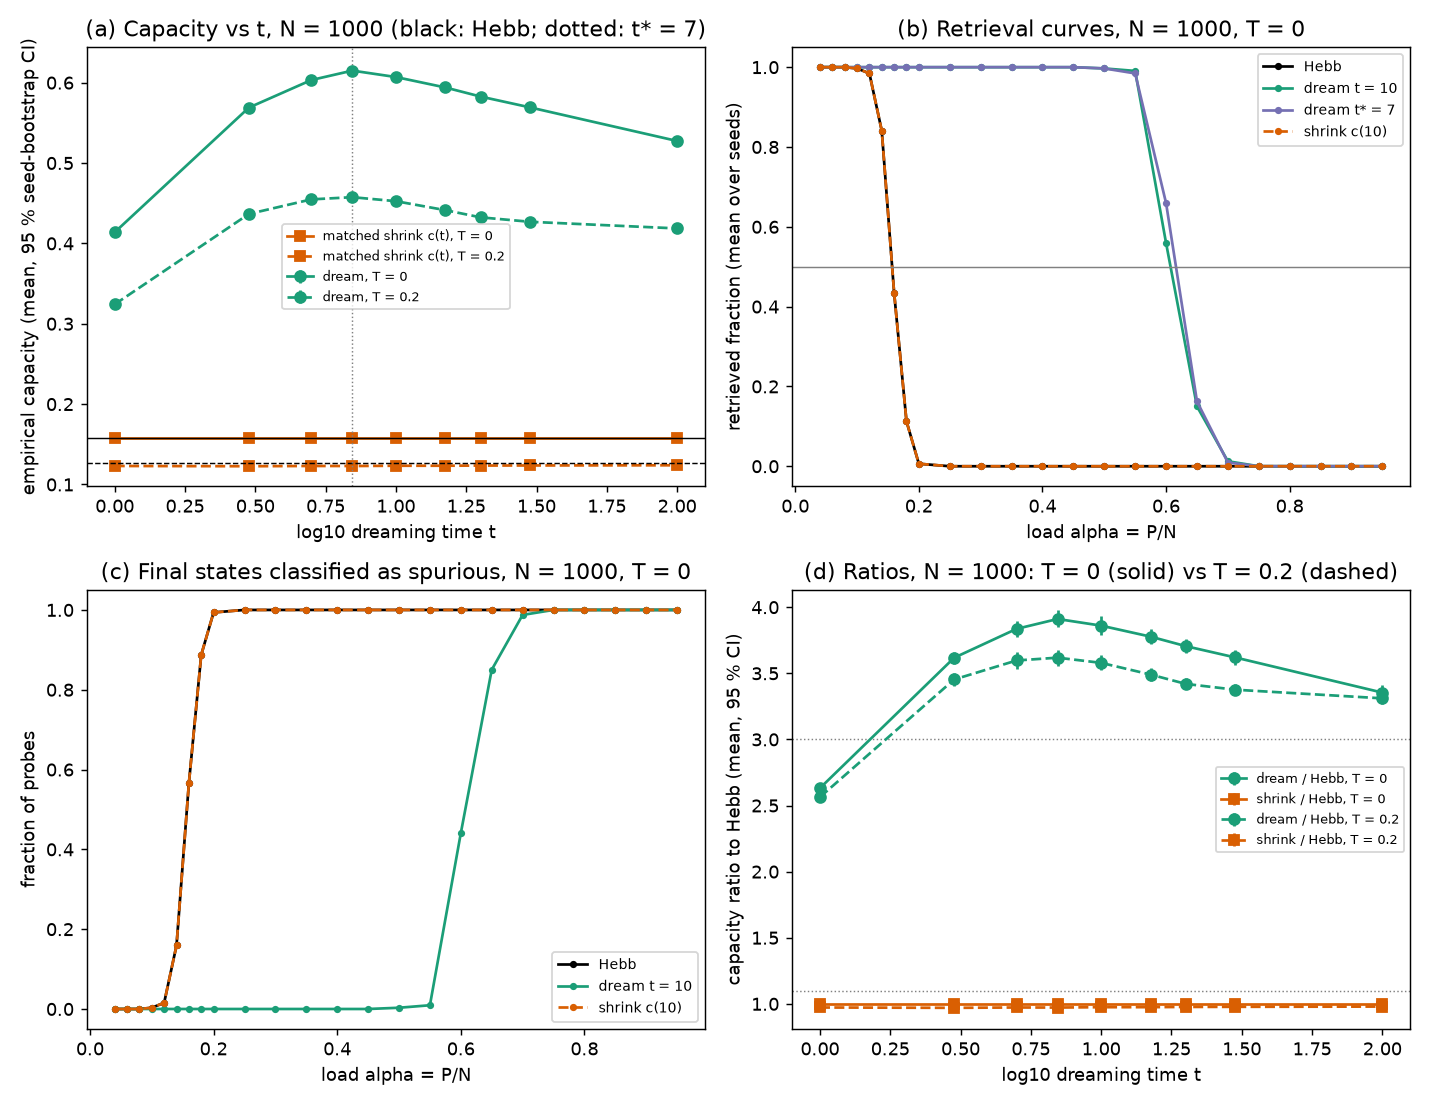
\includegraphics[width=1\linewidth,height=\textheight,keepaspectratio,alt={NH-01
confirmatory run, N = 1\textbackslash,000, seeds 0--9
(results/nh01\_confirmatory/figure.png, byte-identical on the provenance
re-run). (a) Empirical capacity \textbackslash hat\textbackslash
alpha\_c versus dreaming time t for the dreamed kernel (circles) and the
matched uniform-shrink control (squares) at T = 0 (solid) and T = 0.2
(dashed); the horizontal lines are the Hebbian reference; the dotted
vertical line marks t\^{}* = 7. (b) Retrieved fraction versus load
\textbackslash alpha at T = 0 for Hebb, dream t = 10, dream t\^{}* = 7
and shrink c(10). (c) Fraction of spurious final states versus load at T
= 0. (d) Capacity ratio to Hebb with seed-level 95 \% bootstrap
intervals; the dotted lines are the pre-registered thresholds 3.0
(confirmation) and 1.1 (control).}]{figures/figure-confirmatory.png}
\caption{NH-01 confirmatory run, \(N = 1\,000\), seeds 0--9
(\protect\texttt{results/nh01\_confirmatory/figure.png}, byte-identical
on the provenance re-run). (a) Empirical capacity \(\hat\alpha_c\)
versus dreaming time \(t\) for the dreamed kernel (circles) and the
matched uniform-shrink control (squares) at \(T = 0\) (solid) and
\(T = 0.2\) (dashed); the horizontal lines are the Hebbian reference;
the dotted vertical line marks \(t^* = 7\). (b) Retrieved fraction
versus load \(\alpha\) at \(T = 0\) for Hebb, dream \(t = 10\), dream
\(t^* = 7\) and shrink \(c(10)\). (c) Fraction of spurious final states
versus load at \(T = 0\). (d) Capacity ratio to Hebb with seed-level 95
\% bootstrap intervals; the dotted lines are the pre-registered
thresholds 3.0 (confirmation) and 1.1
(control).}\label{fig:confirmatory}
\end{figure}

\subsection{Correlated patterns}\label{correlated-patterns}

{[}\texttt{results/nh01\_correlated/summary.json}{]}, \(N = 1\,000\),
seeds 100--109, 29 640 cells, \(t = 10\) unless stated.

{
\begin{longtable}[]{@{}
  >{\raggedright\arraybackslash}p{(\linewidth - 14\tabcolsep) * \real{0.1250}}
  >{\raggedright\arraybackslash}p{(\linewidth - 14\tabcolsep) * \real{0.1250}}
  >{\raggedright\arraybackslash}p{(\linewidth - 14\tabcolsep) * \real{0.1250}}
  >{\raggedright\arraybackslash}p{(\linewidth - 14\tabcolsep) * \real{0.1250}}
  >{\raggedright\arraybackslash}p{(\linewidth - 14\tabcolsep) * \real{0.1250}}
  >{\raggedright\arraybackslash}p{(\linewidth - 14\tabcolsep) * \real{0.1250}}
  >{\raggedright\arraybackslash}p{(\linewidth - 14\tabcolsep) * \real{0.1250}}
  >{\raggedright\arraybackslash}p{(\linewidth - 14\tabcolsep) * \real{0.1250}}@{}}
\toprule\noalign{}
\begin{minipage}[b]{\linewidth}\raggedright
Level \(m\) (\(q = m^2\))
\end{minipage} & \begin{minipage}[b]{\linewidth}\raggedright
Hebb \(\hat\alpha_c\), \(T = 0\)
\end{minipage} & \begin{minipage}[b]{\linewidth}\raggedright
dream \(\hat\alpha_c\), \(T = 0\)
\end{minipage} & \begin{minipage}[b]{\linewidth}\raggedright
C1 ratio, \(T = 0\)
\end{minipage} & \begin{minipage}[b]{\linewidth}\raggedright
C2′ \(t^*\)
\end{minipage} & \begin{minipage}[b]{\linewidth}\raggedright
Hebb, \(T = 0.2\)
\end{minipage} & \begin{minipage}[b]{\linewidth}\raggedright
C3′ shrink ratio, \(T = 0.2\)
\end{minipage} & \begin{minipage}[b]{\linewidth}\raggedright
Level verdict
\end{minipage} \\
\midrule\noalign{}
\endhead
\bottomrule\noalign{}
\endlastfoot
0 (0) & 0.160 {[}0.158, 0.162{]} & 0.611 {[}0.606, 0.616{]} &
\textbf{3.82 {[}3.77, 3.88{]}} --- confirmed & 7 (seeds: 5--10); drop
0.084 {[}0.079, 0.089{]} --- holds & 0.127 {[}0.125, 0.129{]} &
\textbf{0.979 {[}0.974, 0.984{]}} --- holds & \textbf{confirmed} \\
0.15 (0.0225) & 0.068 {[}0.066, 0.070{]} & 0.616 {[}0.612, 0.619{]} &
\textbf{9.06 {[}8.84, 9.29{]}} --- confirmed & 7 (7--10); drop 0.088
{[}0.085, 0.090{]} --- holds & 0.054 {[}0.053, 0.056{]} & \textbf{0.986
{[}0.979, 0.993{]}} --- holds & \textbf{confirmed} \\
0.30 (0.09) & 0.014 {[}0.014, 0.015{]} (all seeds between loads 0.01 and
0.02) & 0.636 {[}0.633, 0.639{]} & computable but \textbf{not retained}
(all ten denominators positive, bracketed by loads 0.01--0.02;
registered estimate reported in the data) & 10 (7--10); drop 0.103
{[}0.098, 0.108{]} --- holds & 0.007 {[}0.003, 0.011{]}; \textbf{5/10
seeds below grid} (zero sentinel = censored) & \textbf{undefined on 5
seeds}; 0.6 {[}0.2, 1.0{]} on the 5 defined seeds (per-seed 1, 0, 1, 1,
0) & \textbf{inconclusive} (after analysis) \\
\end{longtable}
}

Reading rule for \(m = 0.30\). At \(T = 0\) all ten Hebbian crossings
are bracketed by the loads 0.01 and 0.02 (flags \texttt{ok}), so the
registered ratio is defined, but its magnitude is set by the
interpolation inside that interval and is not retained for quantitative
interpretation. At \(T = 0.2\) five Hebbian estimates are below the grid
and their ratios are undefined; the control statistic in the data uses
only the five defined seeds. The absolute capacities are the robust
reading: the dreamed capacity barely moves with correlation (0.611,
0.616, 0.636) while the Hebbian capacity collapses (0.160, 0.068,
0.014), so the paired absolute gain grows 0.451 {[}0.445, 0.456{]} →
0.548 {[}0.543, 0.552{]} → 0.621 {[}0.618, 0.625{]}. The tagged code
labels C3′ ``holds'' and the level ``confirmed'' in
\texttt{summary.json}, computed on the five defined seeds. This article
reports the level as inconclusive instead: the decision was taken after
the analysis (2026-10-30, commit \texttt{5884927}) and is a
methodological reservation, not a registered rule. Its ground is
censoring and sub-sample selection: with Hebbian retrieval essentially
gone at \(T = 0.2\), a five-seed control cannot discriminate shrink from
Hebb. The registered labels are kept unchanged in the raw outputs. The
pre-registered below-grid rule was written for C1 only; a future
amendment should extend it to C3′ and the load grid below 0.01.

C4 trend: the registered estimate is \(R(0.30) - R(0)\) = 40.6 {[}38.7,
43.2{]}, label \texttt{gain\_increases}. Its magnitude depends on the
interpolation of the small Hebbian denominator at \(m = 0.30\) and the
interval does not account for load-grid resolution; we retain the
increasing direction as a descriptive result only. P4 holds at every
level (0 spurious final states under dreaming at
\(\alpha \in \{0.14, 0.20\}\)); the \(T = 0\) exactness check passed at
every level. \(m = 0\) reproduces the independent- pattern run on new
seeds (3.82 vs 3.86; \(t^* = 7\) in both; shrink 0.979 vs 0.975).

\begin{figure}
\centering
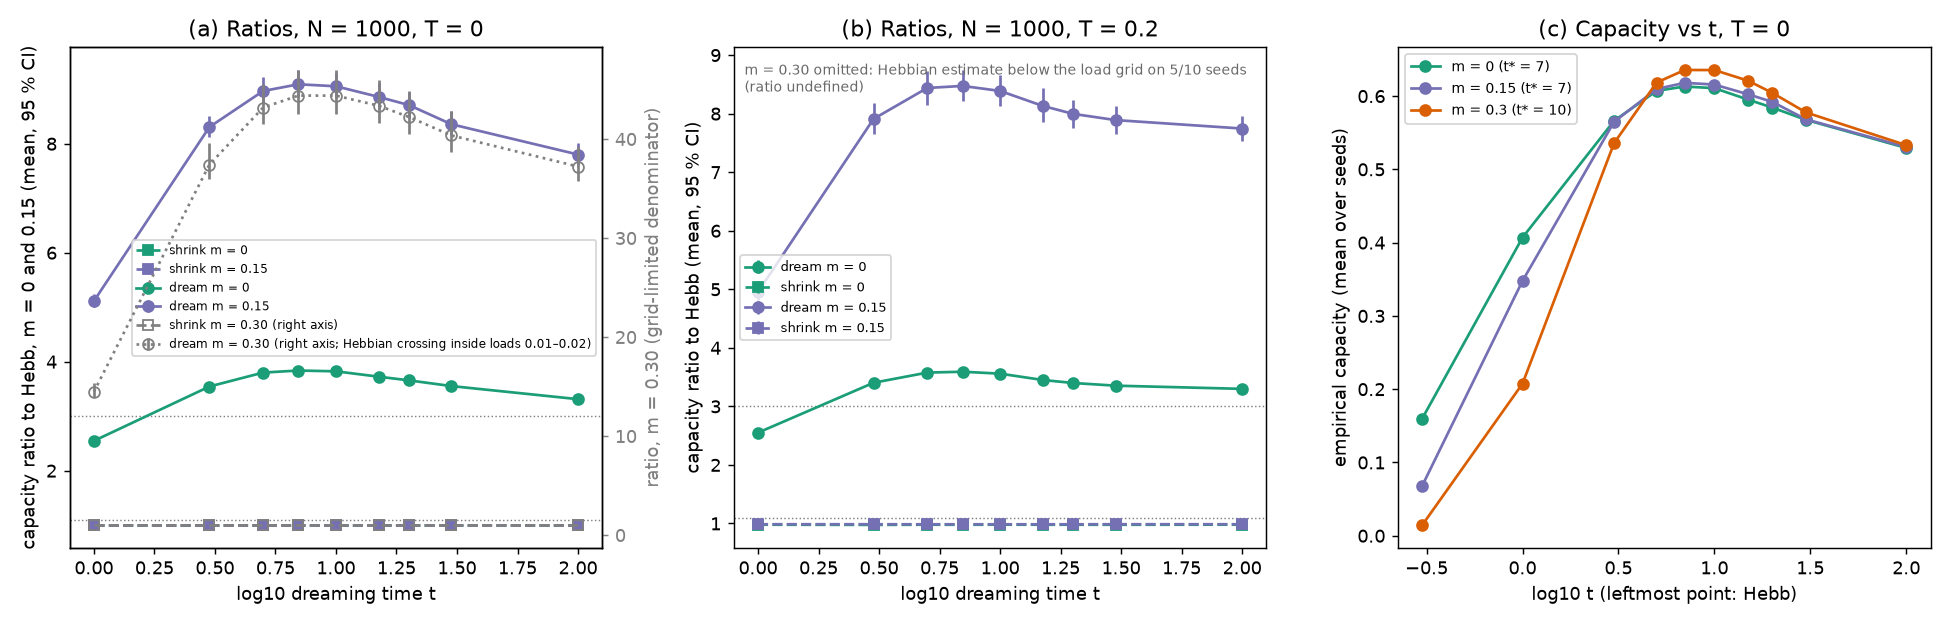
\includegraphics[width=1\linewidth,height=\textheight,keepaspectratio,alt={NH-01
correlated-pattern run, N = 1\textbackslash,000, seeds 100--109
(results/nh01\_correlated/figure.png). (a, b) Capacity ratio to Hebb
versus dreaming time at T = 0 and T = 0.2 for ancestor overlap m
\textbackslash in \textbackslash\{0, 0.15, 0.30\textbackslash\} (dream:
circles; matched shrink: squares). (c) Capacity versus t at T = 0
(leftmost point: Hebb). The figure is the unmodified output of the
tagged code, whose automatic labels read ``confirme'' for all three
levels and draw a ratio curve for m = 0.30; as explained in the text,
the m = 0.30 level is reported as inconclusive: at T = 0 its ratio is
defined but set by the 0.01--0.02 load interval, and at T = 0.2 five of
its ten Hebbian denominators are below the grid, so the m = 0.30 ratio
curves must not be read as a result; the absolute capacities of panel
(c) are the robust reading.}]{figures/figure-correlated.png}
\caption{NH-01 correlated-pattern run, \(N = 1\,000\), seeds 100--109
(\protect\texttt{results/nh01\_correlated/figure.png}). (a, b) Capacity
ratio to Hebb versus dreaming time at \(T = 0\) and \(T = 0.2\) for
ancestor overlap \(m \in \{0, 0.15, 0.30\}\) (dream: circles; matched
shrink: squares). (c) Capacity versus \(t\) at \(T = 0\) (leftmost
point: Hebb). The figure is the unmodified output of the tagged code,
whose automatic labels read ``confirme'' for all three levels and draw a
ratio curve for \(m = 0.30\); as explained in the text, the \(m = 0.30\)
level is reported as inconclusive: at \(T = 0\) its ratio is defined but
set by the 0.01--0.02 load interval, and at \(T = 0.2\) five of its ten
Hebbian denominators are below the grid, so the \(m = 0.30\) ratio
curves must not be read as a result; the absolute capacities of panel
(c) are the robust reading.}\label{fig:correlated}
\end{figure}

\subsection{\texorpdfstring{Internal reproduction of the \(N = 1\,000\)
studies}{Internal reproduction of the N = 1\textbackslash,000 studies}}\label{internal-reproduction-of-the-n-1000-studies}

Both \(N = 1\,000\) runs were re-executed on 2026-10-30 from a fresh
clone checked out at the tag, with the SHA-256 of the executed files
checked against
\texttt{git\ show\ \textless{}tag\textgreater{}:\textless{}file\textgreater{}}
before launch and the tag record fetched from the GitHub API before
launch
{[}\texttt{results/nh01\_confirmatory/provenance-rerun-20261030/},
\texttt{results/nh01\_correlated/provenance-rerun-20261030/}{]}. Result:
\textbf{9 120 / 9 120} and \textbf{29 640 / 29 640} cells identical to
the committed \texttt{cells.jsonl.gz} on every field except the
wall-clock \texttt{task\_seconds} (cells matched by key, NaN compared as
NaN); \texttt{summary.json} identical except its \texttt{run\_meta}
block; \texttt{figure.png} byte-identical (SHA-256 \texttt{3b64a94e…}
and \texttt{de3ee720…}). The re-runs used 2 worker processes instead of
4 for the confirmatory run; the worker count changes only the
scheduling.

\section{Conclusion}\label{conclusion}

Under decision rules fixed before each study's main run, this partial
replication \textbf{supports} the central qualitative claims of
Fachechi, Agliari and Barra within our finite-size protocol: the dreamed
kernel raises the empirical storage capacity of the Hopfield network by
a large factor (3.4--3.9 at \(t = 10\) for independent patterns, \(N\) =
256 to 1 000), leaves no probe classified as spurious at loads 0.14 and
0.20 where the Hebbian network has almost only spurious final states
(which does not establish the absence of spurious attractors elsewhere
in state space), keeps its advantage under thermal noise, and behaves as
the projector rule for large \(t\) (the pilot's \(f = 0\) capacity
estimate is right-censored at \(\alpha =
0.95\) for \(t \ge 10\) --- a 50 \%-retrieval criterion on at most 32
probed patterns, not a test that every stored pattern is a fixed point).
The ratios 3.86 and 9.06 are results of this study, not numbers
published in 2019. On correlated patterns the gain grows with
correlation at \(m \le 0.15\), consistent with the projector limit's
insensitivity to pattern correlations.

Two points go beyond, or qualify, the original. First, the added control
shows that the Frobenius-matched uniform rescalings of the Hebbian
couplings tested here do not reproduce the gain: they are inert at
\(T = 0\) by scale invariance and lower the mean empirical capacity by
2.52 \% at \(T = 0.2\) (seed-bootstrap 95 \% interval 1.80--3.35 \%).
The dreaming effect is a spectral change of the attractor landscape, not
a global downscaling at equal synaptic budget. Second, with the
self-coupling removed and a noisy cue, the finite-size capacity is not
monotone in \(t\): it peaks at \(t^* = 7\) and loses 0.088 {[}0.082,
0.092{]} by \(t = 100\). This does not contradict the mean-field
\(\alpha_c(t)\): our noisy-cue threshold differs from the equilibrium
retrieval boundary of the theory (our \(f = 0\) arm is censored at the
grid maximum, in agreement). We observe a lower empirical capacity at
\(t = 100\) than at the grid optimum \(t = 7\) without measuring basin
sizes or isolating the cause (self-coupling removal, cue noise,
asynchronous dynamics, finite \(N\)). The original article does quantify
retrieval basins, at \(N = 1\,000\) and \(\alpha = 0.05\) under parallel
zero-noise dynamics, and finds them stabilised by dreaming; that
experiment does not cover our higher-load protocol.

What this replication cannot settle: absolute capacities (finite-size,
estimator-dependent), temperatures other than 0 and 0.2, correlation
structures other than a single ancestor, and the \(m = 0.30\) level,
where the Hebbian reference sits at the lower limit of the load grid at
\(T = 0\) and below it on five seeds at \(T = 0.2\). A scale sweep
(nerve-wml\#90) is open and not included here.

\section{Reproducibility}\label{reproducibility}

\begin{itemize}
\tightlist
\item
  \textbf{Code}: \texttt{experiments/nh01\_hopfield\_dream/} of
  https://github.com/hypneum-lab/nerve-wml at tag
  \texttt{prereg-nh01-correlated-20261027} (commit \texttt{df9a1e7};
  contains all three runners). SHA-256 at tag: \texttt{run.py}
  \texttt{35f69477…}, \texttt{confirmatory.py} \texttt{d19aa6d0…},
  \texttt{correlated.py} \texttt{8f269de6…}
  {[}\texttt{results/nh01\_correlated/provenance-rerun-20261030/code\_sha256\_at\_tag.txt}{]}.
  Submission repository: https://github.com/hypneum-lab/rescience-nh01,
  MIT.
\item
  \textbf{Software Heritage}: snapshot
  \texttt{swh:1:snp:01242c8b5873518a503b84a80ce3a302bb69b8a8} (visit
  2026-10-29T10:55:51Z); revisions
  \texttt{swh:1:rev:bc2f838919756a8dc2249e577cc5fac0f21cf0d2} (pilot
  tag), \texttt{swh:1:rev:a000f73addde8ff8ac0f28e72a038ad886848f48}
  (confirmatory tag),
  \texttt{swh:1:rev:df9a1e7634113599c9b38cb4259068a29a5bdd2a}
  (correlated tag), all resolving through the SWH API on 2026-10-31.
\item
  \textbf{Environment}: Python 3.12.15, numpy 2.5.4, matplotlib 3.11.2
  (full freeze in
  \texttt{provenance-rerun-20261030/uv\_pip\_freeze.txt}); no GPU.
  \texttt{OMP\_NUM\_THREADS=OPENBLAS\_NUM\_THREADS=MKL\_NUM\_THREADS=NUMEXPR\_NUM\_THREADS=1}.
\item
  \textbf{Host}: electron-server, 8 × Intel Xeon X5680 (no AVX), Linux
  6.8.0-136, shared with other jobs (load 7--20), \texttt{nice\ 19}.
\item
  \textbf{Commands and wall times} (\texttt{run\_meta.json} of each
  run):

  \begin{itemize}
  \tightlist
  \item
    \texttt{python\ -m\ experiments.nh01\_hopfield\_dream.run\ -\/-workers\ 4\ -\/-out\ results/nh01}
    --- seeds 0--9, started 2026-10-25T08:51:11Z, 1 547 s, 28 080 cells.
  \item
    \texttt{python\ -m\ experiments.nh01\_hopfield\_dream.confirmatory\ -\/-workers\ 4\ -\/-out\ results/nh01\_confirmatory}
    --- seeds 0--9, started 2026-10-25T13:47:22Z (14 s after the tag
    push), 6 951 s, 9 120 cells; re-run with \texttt{-\/-workers\ 2}: 15
    136 s.
  \item
    \texttt{python\ -m\ experiments.nh01\_hopfield\_dream.correlated\ -\/-workers\ 2\ -\/-out\ results/nh01\_correlated}
    --- seeds 100--109, started 2026-10-27T16:48:06Z, 22 866 s, 29 640
    cells; re-run: 30 547 s.
  \item
    \texttt{gzip\ -k\ \textless{}rerun\_dir\textgreater{}/cells.jsonl}
    (the runners write the uncompressed file, the comparator reads
    \texttt{cells.jsonl.gz}), then
    \texttt{python\ -I\ compare\_nh01.py\ \textless{}committed\_dir\textgreater{}\ \textless{}rerun\_dir\textgreater{}\ comparison.json}
    for the cell-by-cell comparison and a reading of its
    \texttt{keys\_equal} and \texttt{summary\_equal\_excl\_run\_meta}
    fields (the script does not set a failure exit status);
    \texttt{-\/-analyze-only} recomputes \texttt{summary.json} and
    \texttt{figure.png} from an existing \texttt{cells.jsonl}.
  \end{itemize}
\item
  \textbf{Seeds}: root 20261025; per-seed streams keyed by (seed, N,
  load, purpose); bootstrap seed 20261025, 10 000 resamples.
\item
  \textbf{Artefacts} (\texttt{SHA256SUMS} in each directory):
  \texttt{results/nh01/}, \texttt{results/nh01\_confirmatory/},
  \texttt{results/nh01\_correlated/} --- each with
  \texttt{cells.jsonl.gz}, \texttt{summary.json}, \texttt{figure.png},
  \texttt{run\_meta.json}, \texttt{run.log}; copied into \texttt{data/}
  of the submission repository. Data DOI: 10.5281/zenodo.23833431
  (nerve-wml v1.10.0, archived 2026-10-31, concept DOI
  10.5281/zenodo.19656342), to be cited with the three
  \texttt{prereg-nh01-*} tags and the SWH snapshot
  \texttt{swh:1:snp:01242c8b…} above.
\item
  \textbf{For reviewers}: unit tests run in seconds; the pilot in
  \textasciitilde26 min on 8 cores; the two \(N = 1\,000\) runs in 2--8
  h depending on workers. Expected outputs are the committed
  \texttt{summary.json} files. The two \(N = 1\,000\) studies were
  reproduced on the original host with exact non-timing cell values and
  identical figure files; on another platform, cell keys and discrete
  outcomes (classifications, flags, sweeps) should match exactly and
  floating-point diagnostics (\texttt{c\_fro}, \texttt{energy\_own}) to
  about \(10^{-12}\), while PNG byte identity is not required. The pilot
  is not covered by the internal re-run.
\end{itemize}
